\documentclass[runningheads]{llncs}


\usepackage[utf8]{inputenc}
\usepackage[numbers, comma, sort]{natbib}
\bibliographystyle{apalike}

\usepackage{amssymb}
\setcounter{tocdepth}{3}
\usepackage{graphicx}
\usepackage{float}


\usepackage{pgfplots}
\usepackage{tikz}
\usetikzlibrary{arrows,backgrounds,positioning}


\usepackage{url}
\urldef{\mailsa}\path|rob@clabs.cc, schubotz@tu-berlin.de|
\newcommand{\todaydate}{\leadingzero{\day}.\leadingzero{\month}.\the\year} 
\newcommand{\keywords}[1]{\par\addvspace\baselineskip
\noindent\keywordname\enspace\ignorespaces#1}

\begin{document}

\mainmatter

\title{Mathematical Language Processing \\ Project}
\titlerunning{MLP}

\author{Robert Pagel \and Moritz Schubotz}
\authorrunning{Pagel, Schubotz}

\institute{Berlin Institute of Technology, Database Systems and Information Management Group,\\
Einsteinufer 17, 10587 Berlin, Germany\\
\mailsa\\
\url{http://www.dima.tu-berlin.de/}}


\maketitle


\begin{abstract}
The \emph{Mathematical Language Processing project} addresses the problem of discovering definition relations between variable symbols and the surrounding text. For machine learning approaches like support vector machines, a labelled text corpus is a prerequisite. Unlike traditional approaches, we propose a strategy for automated data labelling with very limited supervision. We analyse the surface of the surrounding text and track co-occurrences of artifacts within the sentences to extract relations. 
%\keywords{machine learning, text mining, parallel computing}
\end{abstract}


\section{Introduction}


\subsection{Motivation}
Mathematical formulas are a viable source of information for a wide range of scientists. Often those formulas contain variables that are unknown or at least ambiguous to the reader. Therefore, one needs to study the surrounding text to find the relevant definition.

An automatic information retrieval system can be used to reduce the readers effort to understand a formula. Especially students and scientists of other disciplines would profit of such a system.

Unfortunately, we were not able to find a labelled text corpus that annotates variables and their definition. Instead of labelling large amounts of text by hand, we investigate a potential way of automatically labelling large corpora with a set of statistical assumptions. One can derive distributional statistics of the found patterns on a large labelled corpus. This statistics may indicate \emph{overfitting features} and, therefore, help to mitigate dimensionality issues with a classifier \cite{Oommen2008}.

We chose the Wikipedia text corpus as a target because of two facts. First, the mark-up for editing formulas is a subset of \TeX. Therefore, it enables us to collect all variables within the set of formulas in a document. Second, we can leverage the semantic information between mark-up and word tokens, e.g., links to other articles.

The English Wikipedia contains roughly four million articles. Even if we only pick articles containing \texttt{<math/>} mark-up, our processor still needs to compute tens of thousands of articles. Especially when using a maximum entropy \emph{POS} tagger \cite{Rathna96}, like the one in Stanford's NLP framework, one can make use of a parallel processing system to speed up computation.

We will show how the proposed strategy can be implemented in the PACT programming model \cite{Alexandrov2010}.


\subsection{Related Work}
\citeauthor{Quoc2010} (2010) proposed in \cite{Quoc2010} an approach for relating whole formulas to sentences and their describing paragraphs. \citeauthor{Yokoi} (2010) trained a \emph{support vector machine} to extract natural language descriptions for mathematical expressions \cite{Yokoi}.


\section{Relation Discovery}
The basic assumption of our approach is that if two entities take part in a relation, those two co-occurre in the same sentence. This assumption is also used in the \emph{Distant Supervision} \cite{Mintz2008} approach by \citeauthor{Mintz2008} Furthermore, we assume in a scientific document, which contains a specific variable name, there is at least one sentence with such a relation.

The two entities have some characteristics that can be used for filtering. First of all, the relevant variables can be retrieved accurately from \TeX\ formatted formulas (see Section \ref{vr}). The fact that a definition relation consists of two entities and we know that one must be the variable, leads to an obvious conclusion: Sentences without a variable cannot contain a definition relation and can be discarded.
Second, one can assume that the other entity must be a noun or a compound noun. Thus, all words that are not nouns or adjectives describing these nouns, can also be discarded.


\subsection{Numerical Statistics}
As a prerequisite for detecting potential relations, one needs to identify all occurrences of a variable within a document. Our intuition tells us, that the corresponding definition relation entities can be found near the variables. In other words, the distance between a variable and an entity correlates to the probability of being a definition relation.

We translate this into a rating function based on the gaussian curve that takes the entity word positions $p_{1}$ and $p_{2}$ and relates the resulting distance to a value in $[0;1]$.

\begin{equation}
\label{eq:dist}
R_{d}(p_{1}-p_{2}) = R_{d}(d) = \exp\left[-\frac{d^{2}}{2c_{d}^{2}}\right]
\end{equation}

The parameter $c_{d}$ relates to the full width at half maximum. We assume that most of the definition relations span across five words. One might choose $c_{s}$, such that $R_{d}(p_{1},p_{2}) = \frac{1}{2}$ if $\left|p_{2}-p_{1}\right| = 5$. Therefore, $c_{d} = 5 / \sqrt{2\log{2}}$. Please note that this assumption is heavily influenced by the language of the text corpus. 

Not only the distances within one sentence are of interest. Also the sequential order of sentences, containing a variable, carry some viable sources for statistics. Usually, we experiance that an author first introduces a term and uses it in subsequent sentences without necessarily repeating its definition. We assume that this kind of behaviour also applies to the use of variables. Thus, we extend the idea of distance to the sequential order of sentences. Here, the distance is the count $n$ of candidate sentences, beginning at the top of the document.

\begin{equation}
\label{eq:order}
R_{s}(n) = \exp\left[-\frac{n^{2}}{2c_{s}^{2}}\right]
\end{equation}

We define the parameter $c_{s}$ analogous to $c_{d}$ used in Equation \ref{eq:dist}. In our experiments, we expect that most of the definition relations are found within the first three sentences. Thus, $c_{s} = 3 / \sqrt{2\log{2}}$.

\begin{figure}[H]
\centering
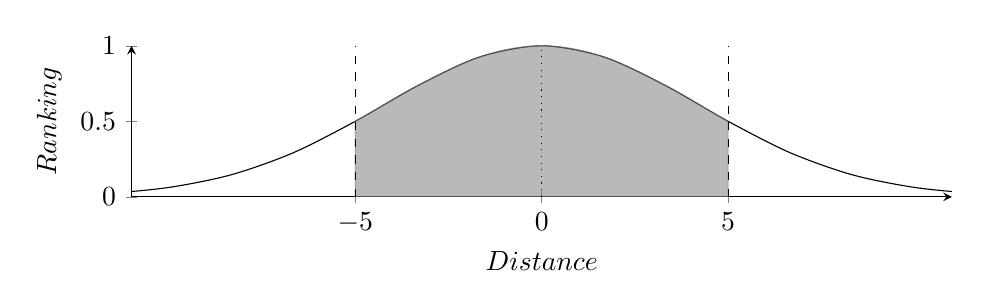
\begin{tikzpicture}
	\begin{axis}[
			axis x line = bottom,
			axis y line = left,
			height=3.5cm, width=12cm,
			xmin=-11, xmax=11,
			ymin=0, ymax=1,
			xtick={-5,0,5},
			ytick={0,0.5,1},
			xlabel=$Distance$,
			ylabel=$Ranking$]
		\addplot [mark=,domain=-20:20,smooth]{e^(-( x^2 / 36.06737602222409 ))};
		\addplot [mark=,domain=-5:5,smooth, gray,fill=gray!90!black,opacity=0.5]{e^(-( x^2 / 36.06737602222409 ))} \closedcycle;
		\addplot [black,dotted] coordinates {(0,0) (0,1)};
		\addplot [black,dashed] coordinates {(5,0) (5,1)};
		\addplot [black,dashed] coordinates {(-5,0) (-5,1)};
	\end{axis}
\end{tikzpicture}
\caption{Curve of the rating function $R_{d}$ with FWHM}
\end{figure}

Furthermore, we take distributional properties into account. The classic tf-idf \cite{Salton86} statistic reflects the importance of a term to a document. Unfortunately, the \emph{inverse document frequency} is not applicable to definition relations. In our approach, the frequency distribution of all terms, that participate in various definition relations is unknown beforehand. Thus, using tf-idf could affect the sensitivity of our rating statistic significantly. E.g., `Hamiltonian' as well as `length' are both valid entities. Obviously, the number of documents (respectively sentences) containing one of these words, within a corpus like Wikipedia, differs a lot.

Therefore, we use the normalized term frequency. $t$ and $w$ are terms. $f$ denotes the raw frequency of a term within a document $d$.

\begin{equation}
	\label{eq:tf}
	\mathrm{tf}(t,d) = \frac{\mathrm{f}(t,d)}{\max\{\mathrm{f}(w,d):w \in d\}}
\end{equation}

We define our ranking statistic as the weighted mean of the rankings defined in Equations \ref{eq:dist}, \ref{eq:order}, and \ref{eq:tf}:

\begin{equation}
	\label{eq:rating}
	\frac{\alpha\cdot\mathrm{R}_{d}+\beta\cdot\mathrm{R}_{s}+\gamma\cdot\mathrm{tf}}{\alpha+\beta+\gamma} \mapsto [0;1]
\end{equation}


\section{Implementation}

\subsection{Overview of the processor}
The MLP processing system \cite{github} is a graph of PACTs, where data flows through. In contrast to other programming models like Map/Reduce, PACTs can operate on multiple inputs. At some point of time, we need an ordered list of tokenized sentences and a list of identified variables, to compute the ranking score. A \emph{CoGroup Contract} takes both lists and computes the subsets, build upon distinct document keys. Finally, a \emph{Reduce Contract} filters out results below a given threshold $\theta$.

\tikzset{actor/.style={
        rectangle,
        minimum size=6mm,
        very thick,
        draw=gray!50!black!50,
        top color=white,
        bottom color=gray!50!black!20
    },
    arrow/.style={
        -latex, thick, shorten <=2pt,shorten >=2pt
    }
}
\begin{figure}[H]
	\centering
	\begin{tikzpicture}[node distance=5mm and 8mm]
		\node (Input) [align=center]{Wiki Dumps};
		\node (DocumentParser) [actor, right=of Input, align=center] {\emph{Map}\\\textbf{Parser}};
		\node (Candidates) [actor, right=of DocumentParser, align=center] {\emph{CoGroup}\\\textbf{Kernel}};
		\node (Sentence) [actor, above=of DocumentParser, align=center] {\emph{Map}\\\textbf{Tagger}};
		\node (Filter) [actor, right=of Candidates, align=center] {\emph{Reduce}\\\textbf{Filter}};
		\node (Output) [right=of Filter,align=center]{Relation\ Candidates};
		\draw[arrow] (Input)--(DocumentParser);
		\draw[arrow] (DocumentParser)--(Sentence);
		\draw[arrow] (DocumentParser)--(Candidates);
		\draw[arrow] (Sentence.east)--(Candidates.north);
		\draw[arrow] (Candidates)--(Filter);
		\draw[arrow] (Filter)--(Output);
	\end{tikzpicture}
\caption{Data flow of the PACT program}
\end{figure}
There are three computation heavy parts in the processor. First, the raw Wikipedia document dumps need to be transformed into plain text. At the same step, the formulas need to be evaluated and replaced by place-holder words. We used the \emph{WikiText} framework of the Mylyn project with a custom builder to transform the document into plain text. For analysing the \TeX \ mark-up in the \texttt{<math/>} tags, \emph{SnuggleTeX} transforms the formulas into their MathML representations, where variable names can be extracted easily. The second computation heavy part is tokenization and tagging of the plain text documents. We used the Stanford maximum entropy tagger with the \emph{WSJ left3words} language model. Finally, the rating for all nouns, contained in all candidate sentences, needs to be calculated.


\subsection{Experiments}

\subsubsection{Variable Retrieval}
\label{vr}
Throughout our experiments we made some observations that had an impact on the accuracy of retrieving the correct set of variables. First of all, people tend to incorrectly use \TeX\ trying to create formulas. I.e., \texttt{\textbackslash text\{log\}} is more often used than the correct operator \texttt{\textbackslash log}. Another problem is that sometimes people use indices as a form of annotation, like $T_{before}$, $R_{A}$, and $R_{B}$. These ambiguities lead to a increased number of false positives.

We took a very conservative approach and preprocessed all formulas. \texttt{\textbackslash text\{\}} blocks along with plain subscriptions will be removed before analysis. Moreover, we created a comprehensive blacklist to improve the results further. Short words like `a' and `i', which are very common, could be easily matched by our processor if a formula contains one of those symbols. Additionally, we blacklist common mathematical operators, constants, and functions.

Because of the fact, that we do not have any annotated test corpora, evaluation has to be performed by hand. Therefore, we took a sample of 30 random documents and counted all matches. The resulting estimates for \emph{recall} and \emph{precision} are 0.99 and 0.86 respectively.



\subsubsection{Tuning}
The weighting parameters $\alpha$, $\beta$, and $\gamma$ in Equation \ref{eq:rating} are used to balance the contribution of all embedded statistics to the overall ranking. But these parameters need to be tuned carefully. Otherwise the results tend to be biased towards one parameter. In other words, if the distance measure $R_{D}$ dominates the other measures, more complex\footnote{in terms of words between both entities, participating in a relation} relations are less likely to be discovered.

The \emph{term frequency} turns out to be the least robust statistic. Usually, the frequency of a specific term co-occurring with a variable name within one document is rather low. Thus, the derived ranking is relatively volatile. In our experiments, we chose $\gamma$ to be 0.75 ($\alpha = \beta = 1$) for a more robust ranking.


\section{Conclusion}
Our experiments showed that combining a POS tagger with numerical statistics about the text surface, can lead to quality results. However, this approach is only applicable under certain conditions. In situations where both parts of a relation are unknown, other methods, especially supervised ones, are better used to bootstrap a language model. Unfortunately, we still need an other labelled test corpus to measure the real performance of a classifier, trained with the derived features.

Apart from the mentioned weighting parameters, the ranking's quality is influenced by two further parameters. These are the assumptions about the parameters $c_{d}$ and $c_{s}$. Balancing all these parameters requires extensive knowledge about the underlying language. These parameters might also be specific for every type of relation. Therefore, this strategy depends heavily on human input and many iterations of tuning.

To further improve the robustness of the \emph{term frequency} measure, one might cluster sets of scientific documents, based on their specific field of research.



\bibliography{mlp-papers}
\end{document}
